\subsection{The \ONn{1} model -- entropy production and irreversibility of RG flows}\label{subsec:0dO1Entropy}
\begin{disclaimer}
	This subsection is based on \ccite{Koenigstein:2021rxj} and contains parts of the unpublished notes~\cite{Koenigstein:fixedPoint}.
	The plots of \ccite{Koenigstein:2021rxj} and the underlying numerical data were produced by A. Koenigstein and numerically cross-checked by my own computations with the KT scheme.
	
	Selected numerical results and accompanying symbolic computations are included in the digital auxiliary file~\cite{Steil:2023zeroDN1}.
	The single thread wall time on an \intel{} for the numeric results of this subsection is only around eight minutes, since we only discuss five \frg{} trajectories.
	
	The introduction of this subsection follows Secs. I and II of \ccite{Koenigstein:2021rxj}.
\end{disclaimer}
In this subsection we will focus on $O(N=1)$ models, \ie{}, a zero-dimensional \ZII{}-symmetric model of a single scalar, as discussed especially at the beginning of this chapter in \cref{sec:0dQFT}.
In the spirit of \cref{paragraph:conservative_form_diffusion}, the limitation to $N=1$ entails, that the flow equation gets purely diffusive as the advective contributions $\propto(N-1)$ vanish.
We are left with the scalar parabolic conservation law,
\begin{align}
	\partial_t U ( t, \sigma ) = \frac{1}{2} \,\frac{1}{r ( t ) + \partial_\sigma^2 U ( t, \sigma )}\, \partial_t r ( t ) = %
	\input{0d/diagrams/SU2model0d-Uflow_00014_1.tex}\, ,	\label{eq:o(1)_wetterich_equation}
\end{align}	
which in primitive form reads
\begin{align}
	\partial_t u ( t, x ) = \, & \alpha[t,\partial_x u ( t, x )] \, \partial_x^2 u ( t, x ) \, ,\label{eq:0ddifprimII}
\end{align}
with the non-linear, strictly positive diffusion coefficient
\begin{align}
	\alpha[t,\partial_x u ( t, x )] \equiv - \frac{\tfrac{1}{2} \, \partial_t r ( t )}{[ r ( t ) + \partial_x u ( t, x ) ]^2} \, ,	\label{eq:diffusion_coefficientII}
\end{align}
\cf{} \cref{eq:0ddifprim,eq:diffusion_coefficient}.
We can identify \cref{eq:0ddifprimII} as a heat equation with non-linear diffusion coefficient \eqref{eq:diffusion_coefficientII}, \cf{} \cref{subsec:hydroDiffusion}.
The present discussion makes our general remarks about functional flow/heat equations in \cref{subsec:RGflow} explicit.
The conservative formulation \eqref{eq:o(1)_wetterich_equation} and interpretation in terms of (numerical) fluid dynamics has tremendous benefits and consequences for understanding and solving this \frg{} flow equation:
	\begin{enumerate}
		\item	The explicit identification of the \frg{} flow \cref{eq:o(1)_wetterich_equation} as a heat equation allows us to directly apply the \cfd{} methods of \cref{sec:conservationLaws} and especially \cref{subsec:hydroDiffusion}.
		\item	An interpretation of \frg{} flow equations as flow equations in the narrow sense of the word makes the dynamics during the flow intuitively understandable.
		The non-linear diffusive contribution (the radial \sigmaMode{}) smears out cusps and jumps in $u ( t, x )$ and corresponds to undirected movement of $u ( t, x )$, depending on the local ``concentration differences'', the gradient $\partial_x u ( t, x )$, via the highly non-linear diffusion coefficient \eqref{eq:diffusion_coefficientII}.
		\item The described dissipative dynamics goes hand in hand with entropy production and irreversibility as discussed in the \cfd{} context in \cref{subsec:hydroDiffusion}.
		We can therefore conclude that the irreversibility of the \rg{} transformations during the \frg{} flow is hard coded in the diffusive character of the flow \cref{eq:o(1)_wetterich_equation}, not only in zero space-time dimensions, but for any dimension and any \qft{}, \cf{}\ \ccite{Zumbach:1994kc,Zumbach:1994kc,Zumbach:1994vg,Zumbach:1993zz}.
		Hence, the rise of entropy during the \frg{} flow might therefore be directly linked to $\mathcal{C}$-/$\mathcal{A}$-theorems.
		This is explained in detail in this subsection in the context of our minimalistic toy model \qft{}.
	\end{enumerate}

To be specific, we shall show that the numerical entropy, which is of utmost importance in the theoretical treatment of \pdes{}, as outlined in \cref{sec:conservationLaws} and especially \cref{subsec:hydroKT}, has a very close connection to an entropy in the \grg{} flow\footnote{In this context we also have to mention the publication~\cite{Cotler:2022fze} by J. Cotler and S. Rezchikov, who were able to interpret the Polchinski equation as an ``optimal transport gradient flow of a field-theoretic relative entropy'', thus establishing a firm and explicit connection between an information-theoretic entropy and \grg{} flows.} and further possible connections to the so-called $\mathcal{C}$-/$\mathcal{A}$-functions, \cf{}\ \ccite{Zamolodchikov:1986gt,Rosten:2010vm,Banks:1987qs,Cardy:1988cwa,Osborn:1989td,Jack:1990eb,Komargodski:2011vj,Curtright:2011qg,Haagensen:1993by,Generowicz:1997he,Forte:1998dx,Codello:2013iqa,Codello:2015ana,Becker:2014pea,Becker:2016zcn} and \cref{subsubsec:c-theorem_irreversibility_entropy} for more details on $\mathcal{C}$-/$\mathcal{A}$-functions.

One of the most important direct consequences of this is, that the same ``(thermodynamic) arrow of time'' or ``thermodynamic time asymmetry''~\cite{Lebowitz:2008} identified by the entropy of a \pde{}, is also present from a \frg{} perspective.

In nature as well as in the \pdes{} that describe our physical world, entropy is produced by diffusion (dissipation) as well as discontinuities of different kinds.
Consequently the evolution of such systems and also their numerical solutions are irreversible and usually only weak solutions are accessible numerically~\cite{Lax1973,Ames:1992,LeVeque:1992,LeVeque:2002,Hesthaven2007,Toro2009,RezzollaZanotti:2013}.
As we will demonstrate in this subsection, the \acrrepeat{tvni} property and related numerical entropy, \cf{} \cref{eq:TVcontinuous} and the subsequent discussions of \cref{sec:conservationLaws}, used to guarantee the stability of numeric solution schemes, can be promoted to a ``physical'' entropy function.
This entropy function shares characteristics with a $\mathcal{C}$-function and its properties transfer from the \pde{} to the \qft{} and vice versa.
Therefore, \grg{} flows are also not reversible.\footnote{Note that similar arguments, which link the dissipative character of \rg{} flow equations to the irreversibility of the \rg{} flow, were already brought up in \ccite{Zumbach:1994vg,Zamolodchikov:1986gt} already before or parallel to the development of the functional \rg{} framework pioneered in \ccite{Wetterich:1992yh}.} This makes the semi-group character of the \rg{}, see, \eg{}, \ccite{deligne1999quantum}, explicit.
This semi-group character manifests very explicitly in Kadanoff's block-spin picture~\cite{Kadanoff:1966wm,Wilson:1971bg,Wilson:1971dh,Wilson:1979qg} \dash{} it is intuitively obvious that the averaging over a set of spins is an irreversible process.
The irreversibility of \grg{} flows is not just an abstract concept, but is present on a practical level in rather simple truncations of the Wetterich equation. 

These statements may have no severe practical implications for studies of, \eg{}, \qcd{} and condensed-matter systems, where the \grg{} flow is in general  followed from small (\uv{} limit) to large length scales (\ir{} limit).
In these cases, the dynamics in the long-range limit is predicted from a given known \uv{} action by integrating out high momentum modes along the ``natural'' \rgtime{}-direction.
However, in situations where \grg{} flows are followed from large to small length scales, such as studies of the asymptotic safety scenario in \qfts{} (see \ccite{Weinberg:1976xy,Weinberg:1996kw,Percacci:2007sz,Weinberg:2009ca,Rosten:2010vm} in general, \ccite{Niedermaier:2006wt,Bonanno:2020bil} for a recent review in the context of (quantum) gravity, and \ccite{Braun:2010tt,Jakovac:2014lqa} for applications in condensed-matter physics), the question of irreversibility of \grg{} flows and the associated production of entropy may indeed be very relevant.

Whereas \frg{} flows are indeed reversible for certain classes of truncations (of the underlying effective action), we shall demonstrate in the present work \dash{} with the aid of simple models \dash{} that it becomes formally impossible to reverse \frg{} flows in cases where no truncations of the effective action are made.
Even more, already for often employed truncation schemes (\eg{}, \lpa{}), we shall see that irreversibility associated with numerical entropy production can already be a manifest feature of \frg{} flows.
Of course, irreversibility of \frg{} flows does not imply, that it is not possible to construct theories, which are valid on all scales.
It only implies, that the search for such theories may in general be more complicated.
We already mentioned in our discussion of \rgcy{} of \cref{subsec:RGconsistency}, that irreversibility of \grg{} flows might complicate \rgct{} reconstructions significantly, \cf{} \cref{eq:rgcEq14rev} and the corresponding discussion.
In any case, generalizations of the arguments presented in our present work may help to provide a fresh view on these aspects (and/or revive some already existing discussions~\cite{Zamolodchikov:1986gt,Zumbach:1993zz,Zumbach:1994kc,Zumbach:1994vg,Rosten:2010vm,Felder:1987,Hasenfratz:1985dm}).

As we shall discuss below, fixed points still play an important role within the fluid-dynamic interpretation of \frg{} flows.
In fact, fixed points can be identified with steady-flow solutions and/or (thermal) equilibrium situations on the level of the rescaled dimensionless flow equations, which have advective and diffusive character.

One major benefit of the connection revealed in this work is that a measure for the irreversibility of the \frg{} flow is explicitly provided via the identification with numerical entropy and especially total variation~\cite{LeVeque:1992,LeVeque:2002,RezzollaZanotti:2013,KTO2-0,HARTEN1983357}.
Hence, the construction and analysis of such a measure, at least in certain truncations, might be greatly simplified.
In the future, this might also help to single out adequate truncation schemes for \frg{} flow equations as those truncations, which maintain the inherently irreversible character of the flow.
We note that observations similar to ours have already been pointed out in \ccite{Rosten:2010vm,Zumbach:1993zz,Zumbach:1994kc,Zumbach:1994vg} for related (partially linearized) flow equations.

The rest of this subsection is organized as follows: Numerical entropy and the \tvni{} property are discussed in detail in \cref{subsubsec:0dO1entropy_c-function_tvd}.
Explicit computations and a detailed analysis of numerical entropy production for our test cases are presented in \cref{subsubsec:0dO1numerical_tests}.
In \cref{subsubsec:c-theorem_irreversibility_entropy}, we discuss the manifestation of a \texorpdfstring{$\mathcal{C}$}{C}-theorem for the zero-dimensional $O(1)$ model, challenges for the generalization to finite $N>1$ in zero dimensions, and we briefly comment on possible generalizations of our findings to higher-dimensional theories.

\subsubsection{(Numerical) entropy and the total variation}\label{subsubsec:0dO1entropy_c-function_tvd}
\begin{disclaimer}
	This subsubsection is based on Sec. III of \ccite{Koenigstein:2021rxj}.
\end{disclaimer}
The \customref{paragraph:entropy}{first part} of this subsubsection deals with the explicit construction of a (numerical) entropy for the conservation law \eqref{eq:o(1)_wetterich_equation}.
This entropy has to be a functional of the conserved quantity $u ( t, x )$ and/or its derivatives\footnote{%
	The purely diffusive character of \cref{eq:o(1)_wetterich_equation} is expected to smoothen $u ( t, x )$ during the \frg{} flow which renders $u ( t, x )$ differentiable (but not necessarily analytic) at least for $0 < t < \infty$. This does not need to be the case for hyperbolic conservation laws where taking derivatives of $u ( t, x )$ has to be handled with great care, \eg{}, around shocks, \ie{}, in a proper weak formulation, see \cref{sec:conservationLaws}.%
} that is monotonically rising during the \frg{} flow.
Monotonicity is explicitly proven for valid initial conditions $U ( t = 0, x )$.
Since $u ( t, x )$ is by definition a function of all couplings of the theory, the (numerical) entropy function might therefore be linked to a zero-dimensional version of $\mathcal{C}$-/$\mathcal{A}$-function.
In fact it might have some practical advantages compared to other approaches toward $\mathcal{C}$-/$\mathcal{A}$-functions studied in literature, since $u ( t, x )$ does not even need to be expandable in explicit couplings at all, but still contains all degrees of freedom.

In the \customref{paragraph:discrete_c_and_tvd}{second part} of this subsubsection, we derive a discrete formulation of this entropy functional and demonstrate that it can be directly related to the \acrrepeatEmph{tv}, \ie{}, the arc-length, of $u ( t, x )$.
Thus providing a link between the total \tvd{}/\tvni{} property \dash{} commonly used in numeric schemes for conservation laws~\cite{HARTEN1983357,Lax1973,KTO2-0} \dash{} and our field theoretical notion of entropy here.

\paragraph{Construction of the (numerical) entropy}\phantomsection\label{paragraph:entropy}\mbox{}\\%
The construction of our (numerical) entropy function is directly inspired by the construction of entropy/energy functionals for the \bbeq{}~\cite{Bateman1915,Burgers1948} or the \heq{}~\cite{Cannon:1984} of \cref{paragraph:BBE} and \cref{paragraph:HE}.

Let $y \in \Reals{}$ and
\begin{align}
	&	s : \Reals{} \to \Reals{} \, ,	\qquad \qquad	y \mapsto s ( y ) \, ,
\end{align}
be a continuously twice differentiable convex function on $\Reals{}$, hence
\begin{align}
	&	s ( y ) \in C^2 ( \Reals{} ) \, ,\qquad \qquad	s^{\prime\prime} ( y ) \geq 0 \, ,	\label{eq:convexity_of_entropy_function}
\end{align}
for all~$y  \in \Reals{}$. 
Furthermore, we require that $s ( y )$ shall not grow faster than $y^2$ for $|y| \rightarrow \infty$, which is explained below. Using $s ( y )$ we define the functional
\begin{align}
	S [ f ( x ) ] \equiv - \int_{-\infty}^{+\infty} \dif x \, s ( f ( x ) ) \, ,	\label{eq:entropy_functional}
\end{align}
which we shall refer to as \textit{entropy functional}.
In general, the bounds of integration are chosen according to the domain of our problem at hand.
Next, we prove that, choosing $f ( x ) = \partial_x u ( t, x )$, \cref{eq:entropy_functional} indeed plays the role of an (numerical) entropy for the \pde{} \eqref{eq:o(1)_wetterich_equation}. 
Hence, it measures, similarly to $\mathcal{C}$-/$\mathcal{A}$-functions for \rg{} flows, the degrees of freedom and irreversibility.
To this end, we explicitly demonstrate that $S [ \partial_x u ( t, x ) ]$ is monotonically increasing during the \frg{} flow, thus being a monotonic function on $t \in [ 0, \infty )$:
\begin{align}
	\dod{}{t} S [ \partial_x u ( t, x ) ] \geq 0 \, .	\label{eq:entropy_rises}
\end{align}
The only further ingredient, which is needed for the proof is the spatial derivative of the flow-equation \eqref{eq:o(1)_wetterich_equation}:
\begin{align}
	\partial_t [ \partial_x u ( t, x ) ] = & - \dod{}{x} \! \bigg( \frac{1}{2} \, \frac{\partial_x^2 u ( t, x )}{[ r ( t ) + \partial_x u ( t , x ) ]^2}\, \partial_t r ( t )  \bigg) \, .
\end{align}
Taking spatial derivatives of $u ( t, \sigma )$ should be allowed at any $t \in ( 0 , \infty )$ because of the smoothening character of the diffusion \dash{} at least in zero space-time dimensions\footnote{\label{footnote:entropyWeakDerivation}%
	The generalization of this argument to higher-dimensional $O(N)$-type models might be delicate, because the non-linear diffusion can also cause non-analyticities in potentials in the \ir{} if these end up in the symmetry broken phase.
	In that case it might be unavoidable to base and repeat the entire discussion using a rigorous weak/integral formulation of the \pdes{} under consideration.%
}.
Only for $t = 0$ the initial condition may violate smoothness, see \cref{subsubsec:zerodICS} for details. 
In the following, we normalize the entropy and subtract the entropy of the initial condition $S [ \partial_x u ( t = 0, x ) ]$, such that this should not spoil any of our subsequent arguments.

Let us now prove \cref{eq:entropy_rises}:
\begin{subequations}\label{eq:dSdtproof}
\begin{align}
\dod{}{t} S [ \partial_x u ( t, x ) ] =\, & - \dod{}{t} \int_{-\infty}^{+\infty} \dif x \, s ( \partial_x u ( t, x ) )=\\*[.2em] % no page break here
	= \,& - \int_{-\infty}^{+\infty} \dif x \, \big( \partial_t [ \partial_x u ( t, x ) ] \big) \, s^\prime ( \partial_x u ( t, x ) ) =	
	\\*[.2em] % no page break here
	= \, & \int_{-\infty}^{+\infty} \dif x \, \bigg[ \dod{}{x} \! \bigg( \frac{1}{2} \, \frac{\partial_x^2 u ( t, x )}{[ r ( t ) + \partial_x u ( t , x ) ]^2}\,\partial_t r ( t )  \bigg) \bigg] \, s^\prime ( \partial_x u ( t, x ) ) =	\\*[.2em] % no page break here
	= \, & \int_{-\infty}^{+\infty} \dif x \, \big[ - \tfrac{1}{2} \, \partial_t r ( t ) \big]  \, \frac{[\partial_x^2 u ( t, x )]^2}{[ r ( t ) + \partial_x u ( t , x ) ]^2} \, s^{\prime\prime} ( \partial_x u ( t, x ) ) +\notag\\*[.1em] % no page break here
	&\qquad\qquad\qquad+\bigg[ \frac{1}{2} \, \frac{\partial_x^2 u ( t, x )}{[r ( t ) + \partial_x u ( t , x )]^2}\, \partial_t r ( t )  \, s^{\prime} ( \partial_x u ( t, x ) ) \bigg]_{-\infty}^{+\infty}	\label{eq:dSdtproofD}\\*[.2em] % no page break here
	=\,& \int_{-\infty}^{+\infty} \dif x \,\big[ - \tfrac{1}{2} \, \partial_t r ( t ) \big] \, \frac{[\partial_x^2 u ( t, x )]^2}{[ r ( t ) + \partial_x u ( t , x ) ]^2}\, s^{\prime\prime} ( \partial_x u ( t, x ) )\ge 0\,\quad \square{}.  \label{eq:dSdtproofE}
\end{align}
\end{subequations}
where the sought after inequality in \cref{eq:dSdtproofE} follows from the facts, that the first term in \cref{eq:dSdtproofD} is positive and the surface term in \cref{eq:dSdtproofD} vanishes.
This can be reasoned by analyzing both terms in \cref{eq:dSdtproofD} separately.
	\begin{enumerate}
		\item	We note that all factors in the integrand of the first term are greater or equal to zero: For the regulator insertion, we have 
			\begin{align}
				- \tfrac{1}{2} \, \partial_t r ( t ) \geq 0 \, ,
			\end{align}
		because $r ( t )$ is a monotonically decreasing function. The numerator and the denominator are obviously positive. In fact, for the denominator of the fraction
			\begin{align}
				r ( t ) > \partial_x u ( t, x ) \, ,
			\end{align}
		for all $t$ anyhow, as long as the initial condition $u(t=0,x)$ and the \uv{} scale $\Lambda$ are chosen accordingly, \cf{} \cref{eq:LambdaMin2} of \cref{paragraph:ONRGconsistency}. Finally,
			\begin{align}
				s^{\prime\prime} ( \partial_x u ( t, x ) ) \geq 0 \, ,
			\end{align}
		holds by construction according to \cref{eq:convexity_of_entropy_function}.
		
		In total, we find that the integrand of the first term is always greater or equal to zero, which directly transfers to the integral itself.
		
		\item	For the second term, we first use that, for large $| x |$, the potential $U ( t, x )$ and all its derivatives do not change during the \frg{} flow, as we have elaborated and demonstrated at length in the previous \cref{subsec:0dONresults}.
		Furthermore, we use that $s ( y )$ maximally grows like $y^2$ for $|y| \rightarrow \infty$ by definition. 
		This implies that its derivative $s^\prime ( y )$ increases asymptotically as $y^1$ at most. 
		Additionally, we use that $U ( t, x )$ is at least proportional to $x^2$ for $|x| \rightarrow \infty$ in order to have well-defined expectation values \eqref{eq:ON_expectation_value}. Consequently, we have to distinguish two scenarios.
		
		If $U ( t, x ) \sim x^2$ for large $|x|$, the second term vanishes identically, due to the third spatial derivative of $U ( t, x )$, namely $\partial_x^2 u ( t, x )$, in the numerator. 
		
		Otherwise, if $U ( t, x )$ grows faster than $x^2$ for large $|x|$, the denominator $[ r ( t ) + \partial_x u ( t, x ) ]^2$ will always grow faster than the product $[\partial_x^2 u ( t, x )] \, s^\prime ( \partial_x u ( t, x ) )$ for $|x| \rightarrow \infty$.
		
		Hence we ultimately conclude that the second term always vanishes, provided that the initial conditions come with the assumed large-$|x|$-asymptotic behavior.
	\end{enumerate}
In summary, we have shown that the statement of \cref{eq:entropy_rises} holds on account of the proof~\eqref{eq:dSdtproof}, which promotes $S$ to an entropy (functional) of our system that can only increase.\bigskip

For what follows, we choose the twice differentiable convex function $s ( y ) = y^2$. This implies
\begin{align}
	S [ \partial_x u ( t, x ) ] = - \int_{-\infty}^{+\infty} \dif x \, [ \partial_x u ( t, x ) ]^2 \, .	\label{eq:entropy_func}
\end{align}
$S$ can be viewed as measure for the richness of structure of the potential \dash{} the information encoded in the potential \dash{} by integrating the square of the gradient of $u(t,x)$ over all positions $x$ in field space.

With the definition \eqref{eq:entropy_func} the following practical problem arises: For practical purposes $S [ \partial_x u ( t, x ) ]$ formally diverges at any time $t$ because $\partial_x u ( t, x )$ is at least constant for $|x| \rightarrow \infty$.
This problem can be cured, by subtracting the entropy $S [ \partial_x u ( t = 0, x ) ]$ of the initial condition.
Since $u ( t, x )$ does not change for large $|x|$ during the entire \frg{} flow, the infinite but constant contributions cancel and we can observe the relative rise in entropy.
This should be a valid approach, since we are only interested in these relative changes anyhow.
We therefore define and consider the normalized entropy
\begin{align}
	\mathcal{C} [ \partial_x u ( t, x ) ] = S [ \partial_x u ( t, x ) ] - S [ \partial_x u ( t = 0, x ) ] \, , \label{eq:Cdef}
\end{align}
which is finite.
Potential subtleties regarding the finiteness of $S$ and $\mathcal{C}$ will be discussed in \cref{paragraph:sc4O1}.
The alphabetic character ``$\mathcal{C}$'' is chosen because this function quantifies irreversibility similarly to $\mathcal{C}$-/$\mathcal{A}$-functions.
We are aware of the fact that a real $\mathcal{C}$-/$\mathcal{A}$-function should be based on the dimensionless rescaled flow equation.
This issue is discussed in \cref{subsubsec:c-theorem_irreversibility_entropy}.

\Cref{eq:Cdef} for the $\mathcal{C}$-function makes the loss of information/richness of structure of the effective potential $u(t,x)$ during \frg{} time evolution explicit. $\mathcal{C}$ monotonically increases with \frg{} time $t$ because the richness of structure/information decreases with $t$.
A loss of information about a system (effective potential $u(t,x)$) during \rgtime{} evolution goes hand in hand with the impossibility to reconstruct/recover earlier states of the system (which had more information) and thus the \rgtime{} evolution is irreversible.
In the present setup the purely diffusive flow equation of the zero-dimensional $O(1)$ model is responsible for this loss of information as large gradients are smeared out by diffusion during \rgtime{} evolution, \cf{} \cref{subsubsec:0dO1numerical_tests} for explicit numerical examples.

\paragraph{Discrete formulation and relation to the \tvni{} property}\phantomsection\label{paragraph:discrete_c_and_tvd}\mbox{}\\%
In this paragraph we discuss a discretized version of \cref{eq:Cdef}, which is suited for practical computations.
In the following and \wlogA{} we consider a \fv{} discretization of $u ( t, x )$ in $x$ with $n$ volume cells of constant width $\Delta x$, centered at $x_i$, $i \in \{ 0, 1, \ldots, n - 1\}$, see \cref{subsec:hydroFV} for details.
Recall that the \frg{} flow in this setup is described by the temporal evolution of the $n$ volume averages $\bar{u}_i ( t )$, which are formally defined as the spatial averages of $u ( t, x )$ over $[ x_{i - \ttfrac{1}{2}}, x_{i + \ttfrac{1}{2}} ]$, where $x_{i \pm \ttfrac{1}{2}} \equiv x_i \pm \tfrac{\Delta x}{2}$.
For the purpose of calculating $\mathcal{C} [ \partial_x u ( t, x ) ]$, we reconstruct the first derivatives from the set of volume averages $\{\bar{u}_i(t)\}$ by a first-order \fd{} forward stencil,
\begin{align}
	\partial_x u ( t, x_i ) = \frac{\bar{u}_{i + 1} ( t ) - \bar{u}_{i} ( t )}{\Delta x} + \order (\Delta x) \, .	\label{eq:centeredDifferences}
\end{align}
For the scope of this work this has proven sufficient since the purely diffusive character of the \pde{} smoothens $u ( t, x )$.
However, for non-smooth/non-differentiable initial conditions at $t = 0$, such as \cref{eq:testing_scenario_non-analytic_quadaratic_asymptote} and \eqref{eq:testing_scenario_4} of our numeric examples, a naive \fd{} stencil is of course generically ill-conditioned at the discontinuities\footnote{
	Similar discussions will arise in higher space-time dimensions, \eg{}, in models where the \frg{} flows ends in a symmetry broken phase with a non-analytic \ir{}-potential. 
	Coming back to a related comment made in an earlier footnote~\ref{footnote:entropyWeakDerivation}: such generalizations might require a retracing of the current discussion using a proper weak formulation and in context of \cref{eq:centeredDifferences} probably a limiting procedure like the \muscl{} reconstruction \eqref{eq:FVuxjn}.
}.
As a direct consequence, the absolute value of $S [ \partial_x u ( t = 0, x ) ]$ strongly depends on the explicit discretization points and the ``capturing of the discontinuity'' in the respective volume cells.
For $t \rightarrow \infty$ (as a direct consequence of the \cmwhTheoremWithRefs{}, \cf{} \MWApp{}), $u ( t, x )$ is smooth and the \fd{} approximation is well-behaved as long as $\Delta x$ is not too small.
We conclude that the absolute values of our entropy function \eqref{eq:Cdef} will strongly depend on $\Delta x$ for non-differentiable initial conditions in the \ir{} because we use $S [ \partial_x u ( t = 0, x ) ]$ as normalization, while the qualitative behavior (monotonic rise) is independent of the discretization, which is also true for the discrete total variation \eqref{eq:TVdiscrete}. 
For the smooth initial conditions \eqref{eq:testing_scenario_phi4} and \eqref{eq:testing_scenario_phi6}, we observed little dependence of the absolute values of the $\mathcal{C}[\partial_x u ( t, x )]$ on $\Delta x$, as expected.

We use a grid with the first volume cell of the computational domain centered at zero, $x_0 = 0$, and the last centered at a finite $x_\mathrm{max}$, hence $x_{n - 1} = x_\mathrm{max}$. $x_\mathrm{max}$ is chosen large enough, such that $u ( t, x_\mathrm{max} ) = u ( t = 0, x_\mathrm{max} )$ holds to a sufficient level for all $t$, \cf{} our discussion in \cref{subsec:0dONresults} as well as \ccite{Grossi:2019urj,Pangon:2009pj,Borchardt:2015rxa,Caillol:2012zz}.
This enables a computation of $\mathcal{C} [ \partial_x u ( t, x ) ]$ considering only $x \in [ - x_\mathrm{max}, + x_\mathrm{max} ]$ since the difference 
\begin{align}
S [ \partial_x u ( t, x ) ] - S [ \partial_x u ( t = 0, x ) ]
\end{align}
practically vanishes for $|x|\geq x_\mathrm{max}$.
We therefore study the following quantity:
\begin{align}
	\mathcal{C} [ \partial_x u ( t, x ) ] = \, & - 2 \int_{0}^{x_\mathrm{max}} \dif x \, \big[ \partial_x u ( t, x ) \big]^2 + 2 \int_{0}^{x_\mathrm{max}} \dif x \, \big[ \partial_x u ( t = 0, x ) \big]^2\,,	
\end{align}
leveraging the \ZII{} symmetry of the problem at hand.
Inserting \cref{eq:centeredDifferences} and performing the integrals over the constant segments in the volume cells leads to our semi-discrete formulation
\begin{align}
	\mathcal{C} [ \{\bar{u}_j(t)\} ] = \, & - \frac{2}{\Delta x} \Bigg( \sum_{j = 0}^{n-1} \frac{[ \bar{u}_{j + 1} ( t ) - \bar{u}_{j} ( t ) ]^2}{( 1 + \delta_{j,0} + \delta_{j,n-1} ) } - \sum_{j = 0}^{n-1} \frac{ [ \bar{u}_{j + 1} ( 0 ) - \bar{u}_{j} ( 0 ) ]^2}{( 1 + \delta_{j,0} + \delta_{j,n-1} )} \Bigg) \, ,	\label{eq:Cdiscrete}
\end{align}
where the factor $(1+\delta_{j,0}+\delta_{j,n-1})$ accounts for the fact that we only integrate over the right half of the first and the left half of the last volume cell. 

Recall that practical computations of solutions to the \pde{} \eqref{eq:o(1)_wetterich_equation} on the compact interval $x \in [ 0, x_\mathrm{max} ]$ require carefully chosen boundary conditions~\cite{Koenigstein:2021syz,Steil:2021cbu} to be consistent with solutions of the pure initial value problem posed by \cref{eq:o(1)_wetterich_equation} on the interval $x \in ( - \infty, + \infty )$~\cite{Borchardt:2015rxa,Borchardt:2016pif}.
In the present \fv{} setup we implement boundary conditions with ghost cells, see \cref{eq:phi0BC0,eq:phi0BCinf} of \cref{subsec:boundary_conditions_finite_volume} for details.
For the computation of $\mathcal{C} [ \{ \bar{u}_i ( t ) \} ]$ we require only the ghost-cell average $\bar{u}_{n} ( t ) = 2 \bar{u}_{n-1} ( t ) - \bar{u}_{n-2} ( t )$ as well as the cell averages at $x_i$ for $i \in \{ 0, 1, \ldots, n - 1 \}$. \bigskip

The entropy functional $S [ \partial_x u ( t, x ) ]$ of \cref{eq:entropy_func} discussed in this subsection is closely related to the \acrrepeatEmph{tv}~\cite{HARTEN1983357} \dash{} the arc length \dash{} of the solution $u ( t, x )$, which we introduced in the context of \fv{} methods and \cfd{} in \cref{subsec:hydroKT}, \viz{} in \cref{eq:TVcontinuous,eq:TVdiscrete}.
For a single component system on the (computational) interval $[ 0, x_\mathrm{max} ]$ \cref{eq:TVcontinuous} reads
\begin{align}
	\mathrm{TV} [ \partial_x u ( t, x ) ] \equiv \int_0^{x_\mathrm{max}} \dif x \, | \partial_x u ( t, x ) | \, .	\label{eq:TVcontinuousO1}
\end{align}
The \tv{} qualitatively differs only by a global sign from the entropy functional $S$, where the sign used for the \tv{} is compatible with the mathematical convention for (numerical) entropy.
The use of the absolute value $| \partial_x u ( t, x ) |$ in \cref{eq:TVcontinuousO1} instead of the square $[ \partial_x u ( t, x ) ]^2$ used for $S$ presents only as quantitative difference, which is not of any practical relevance in this work.
On a \fv{} grid, a discretized version of \cref{eq:TVcontinuousO1} is given by
\begin{align}
	\mathrm{TV} [ \{ \bar{u}_j ( t ) \} ] \equiv \sum_{j = 0}^{n-1} | \bar{u}_{j+1} ( t ) - \bar{u}_{j} ( t ) | \, ,	\label{eq:TVdiscreteO1}
\end{align}
where a first-order forward \fd{} stencil is used to discretize the first derivative, \cf{} \cref{eq:TVdiscrete}.

We discussed the \tv{} and the \tvni{} property of conservation laws in \cref{subsec:hydroKT,subsec:hydroAdvection,subsec:hydroDiffusion} and discussed $\mathcal{C}_\mathrm{TV}$ of \cref{eq:TVDentropy} as a numerical entropy and measure linked to the irreversibility of non-linear convection equations.
The flow \cref{eq:o(1)_wetterich_equation} under consideration in this subsubsection is a non-linear, parabolic pure diffusion equation and the construction of the normalized entropy functional $\mathcal{C}$ of \cref{eq:Cdef} can be adapted to prove directly that solutions of the flow \cref{eq:o(1)_wetterich_equation} are in fact \tvni{}.

\begin{table}[t]
	\centering
	\caption{\label{tab:sc_o1_2_point_functions_exact}%
		The table lists the ``exact'' results for $\Gamma^{(2)}$ of the $O(1)$ model (second column) for the various \uv{} initial potentials of our test cases (first column), which are calculated by a brute-force, high-precision one-dimensional numerical integration of the expectation value $\langle \vec{\phi}^{\, 2} \rangle$ from \cref{eq:ON_expectation_value} using \textit{NIntegrate} in \WAMXIIwR{} with a \textit{PrecisionGoal} and \textit{AccuracyGoal} of $10$, \cf{} \cref{tab:sc_1_n_point_functions_exact,tab:sc_2_n_point_functions_exact,tab:sc_3_n_point_functions_exact,tab:sc_4_n_point_functions_exact}. Here, we shall present the first ten digits. The last column lists the relative errors of the numerical solution of the purely diffusive \frg{} flow equation obtained with the second-order accurate \ktScheme{} using the parameters listed in the corresponding \cref{fig:sc_i_on=1_n=800_xmax=10_lambda=1.0e6_tir=60_rg_flow,fig:sc_ii_n_on=1_n=800_xmax=10_lambda=1.0e12_tir=60_rg_flow,fig:sc_ii_p_on=1_n=800_xmax=10_lambda=1.0e12_tir=60_rg_flow,fig:sc_iii_on=1_n=800_xmax=10_lambda=1.0e12_tir=60_rg_flow,fig:sc_iv_on=1_n=800_xmax=10_lambda=1.0e8_tir=60_rg_flow}, see also \cref{subsec:0dONresults} for a detailed discussion of such errors.
	}
	\vspace{\TableAbovecaptionskip}
	\renewcommand{\arraystretch}{1.15}
	\begin{tabular}{l c c}
		\toprule
		\uv{} potential													&	$\Gamma^{(2)}$		&	$| \Gamma^{(2)}_\mathrm{FRG}/\Gamma^{(2)} - 1 |$		\\
		\midrule
		\cref{eq:testing_scenario_non-analytic_quadaratic_asymptote}	&	$0.1768130358$		&	$6.0 \cdot 10^{-6}$\\
		\cref{eq:testing_scenario_phi4} (negative mass)					&	$0.1995098930$		&	$1.1 \cdot 10^{-5}$		\\
		\cref{eq:testing_scenario_phi4} (positive \kern0.3em mass)					&	$1.3324252475$		&	$1.4 \cdot 10^{-5}$		\\
		\cref{eq:testing_scenario_phi6}								&	$0.1740508127$		&	$2.5 \cdot 10^{-5}$		\\
		\cref{eq:testing_scenario_4}									&	$0.2046977422$		&	$5.8 \cdot 10^{-6}$\\
		\bottomrule
	\end{tabular}
\end{table}
\FloatBarrier
\subsubsection{Numerical entropy production in zero-dimensional models}\label{subsubsec:0dO1entResults}
\begin{disclaimer}
	This subsubsection is based on Sec. IV of \ccite{Koenigstein:2021rxj}.
\end{disclaimer}
\label{subsubsec:0dO1numerical_tests}
In this subsubsection we present explicit numerical results for the \frg{} flows of the (numerical) entropy function \eqref{eq:Cdef} for some selected zero-dimensional $O(1)$ models differing by their action \dash{} \uv{} initial condition for the \frg{} flow.
As explicit examples, we choose the test cases from \cref{subsec:0dONresults} with their established numerical and model parameters.
The following paragraphs
\begin{itemize}
	\item \customref{paragraph:sc1O1}{Test case I: Non-analytic initial condition},
	\item \customref{paragraph:sc2O1}{Test case II: \texorpdfstring{$\phi^4$}{phi**4} potential},
	\item \customref{paragraph:sc3O1}{Test case III: \texorpdfstring{$\phi^6$}{phi**6} potential},
	\item \customref{paragraph:sc4O1}{Test case IV: The \texorpdfstring{$\sigma = 0$}{sigma=0} boundary},
\end{itemize}
contain discussions for the zero-dimensional $O(1)$ model with the respective \ics{} \eqref{eq:testing_scenario_non-analytic_quadaratic_asymptote}, \eqref{eq:testing_scenario_phi4}, \eqref{eq:testing_scenario_phi6}, and \eqref{eq:testing_scenario_4} and are based on Secs. IV. A\dash{}D of \ccite{zerod2}.
For the sake of completeness and as proof of reliability of our numerical scheme and the choice of our numerical parameters, we provide a comparison in \cref{tab:sc_1_n_point_functions_exact} between numerical results for the \ipi{} two-point-function $\Gamma^{(2)}$ calculated via the solution of the flow equation \eqref{eq:o(1)_wetterich_equation} with the \ktScheme{} and ``exact'' results calculated via expectation values \eqref{eq:ON_expectation_value} from the partition function.
Note that all plots of the entropy in this subsubsection are based on a direct implementation of \cref{eq:Cdiscrete}.

\fullWidthTwoSubFigures%
	[!t] % Placement
	{%
		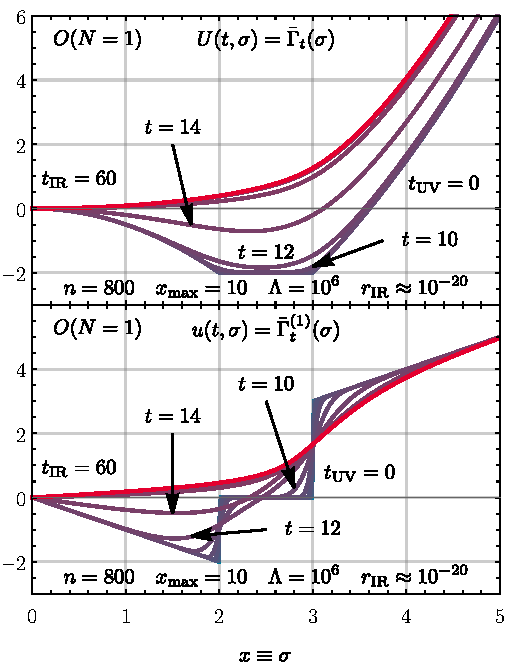
\includegraphics[width=\subcaptionFigureWidth]{0d/figures/sc_i_on=1_n=800_xmax=10_lambda=1.0e6_tir=60_rg_flow.pdf}
		\caption{\frg{} flow of the effective potential $U ( t , \sigma )$ (upper panel) and its derivative $u ( t , \sigma ) = \partial_\sigma U ( t , \sigma )$ (lower panel)}
		\label{fig:sc_i_on=1_n=800_xmax=10_lambda=1.0e6_tir=60_rg_flow}%
	}%
	{
		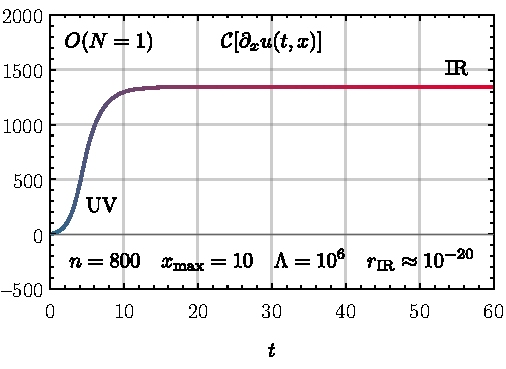
\includegraphics[width=\subcaptionFigureWidth]{0d/figures/sc_i_on=1_n=800_xmax=10_lambda=1.0e6_tir=60_entropy_flow.pdf}
		\caption{\frg{} flow of the numerical entropy $\mathcal{C} [ \partial_x u ( t, x ) ]$}%
		\label{fig:sc_i_on=1_n=800_xmax=10_lambda=1.0e6_tir=60_entropy_flow}%
	} % left figure
	{%
		\caption{
			\frg{} flow of the effective potential and its derivative on the top \subref{fig:sc_i_on=1_n=800_xmax=10_lambda=1.0e6_tir=60_rg_flow} and corresponding flow of the numerical entropy below  \subref{fig:sc_i_on=1_n=800_xmax=10_lambda=1.0e6_tir=60_entropy_flow} for the zero-dimensional \ONn{1} model with initial condition \cref{eq:testing_scenario_non-analytic_quadaratic_asymptote}.
			{Blue} color is associated to the \uv{} and {red} color to the \ir{}.
			We used the exponential regulator \cref{eq:exponential_regulator} with \uv{} scale $\Lambda = 10^6$.
			The lower panel in \subref{fig:sc_i_on=1_n=800_xmax=10_lambda=1.0e6_tir=60_rg_flow} is identical to the upper panel in \cref{fig:sc_i_on_1_10_100_n_800_xmax_10_lambda_1e6_tir_60_rg_flow}.
			\fromFigs{1 and 2}{zerod2}
		}\label{fig:sc_i_on=1_n=800_xmax=10_lambda=1.0e6_tir=60}
		\vspace{2cm}
	}%
\FloatBarrier
\paragraph{Test case I: Non-analytic initial condition}\phantomsection\label{paragraph:sc1O1}\mbox{}\\%
We begin our discussion of $O(1)$ models with test case I \eqref{eq:testing_scenario_non-analytic_quadaratic_asymptote}, recall \cref{fig:sc_i_uv_initial_condition} for a visualization of this \ic{}.
The \frg{} flow of $u ( t, x )$ for $N=1$ is presented in \cref{fig:sc_i_on=1_n=800_xmax=10_lambda=1.0e6_tir=60_rg_flow}.

The diffusive character of the \sigmaMode{} is clearly visible from the fact that it smoothens the discontinuities at $x = 2$ and $x = 3$, without any directed propagation (advection) of the conserved quantity $u ( t, x )$. 
Recall that the system has to restore the \ZII{} symmetry in the ground state as dictated the \cmwhTheoremWithRefs{}.
In particular, the potential has to become convex~\cite{Wipf:2013vp,Fujimoto:1982tc}.
This can be directly observed in the plot of the \frg{} flow and read off from \cref{tab:sc_o1_2_point_functions_exact} \dash{} the two-point function is positive at $\sigma = 0$.\bigskip
	
In \cref{fig:sc_i_on=1_n=800_xmax=10_lambda=1.0e6_tir=60_entropy_flow} we present the \frg{} flow of the (discretized numerical) entropy function for our first test case.

As expected from our discussion in \cref{subsubsec:0dO1entropy_c-function_tvd}, the entropy grows monotonically.
It increases by two orders of magnitude starting at zero in the \uv{} until it reaches (again) a plateau in the \ir{}.
We find that the entropy grows most when the regulator \eqref{eq:exponential_regulator} reaches the model scales.
Loosely speaking, this is where most of the dynamics takes place, see \cref{fig:sc_i_on=1_n=800_xmax=10_lambda=1.0e6_tir=60_rg_flow} (approximately between $t \approx 4$ and $t \approx 8$).
This is the \rgtime{} frame in which the diffusion smears out the discontinuities.
From a fluid- and thermodynamic perspective and directly on the level of the \pde{}, the whole process is intuitively understandable: Diffusion goes hand in hand with strong dissipation and a loss of information about the initial state of the system \dash{} the \uv{}, \cf{} \ccite{Zamolodchikov:1986gt,Zumbach:1994vg}.
This is directly comparable to heat conduction, where the information about the initial temperature distribution gets lost during the flow toward ``thermal'' equilibrium~\cite{Cannon:1984,LeVeque:1992,Lebowitz:2008} as discussed in our introduction of the linear \heq{} in \cref{subsec:hydroDiffusion}.

In the \frg{} framework, this translates to integrating out degrees of freedom from the \uv{} to the \ir{} and a growth in the number of coupling constants in $U ( t, \sigma )$, which is directly related to the growth of entropy.
The entropy plateau in the \ir{} is identified with the interacting \ir{} regime and an ``thermal'' equilibrium on the level of the diffusive \pde{}, whereas a plateau in the \uv{} is associated with a Gaussian \uv{} fixed point~\cite{Zinn-Justin:2010,ZinnJustin:2002ru}.
As expected the entropy stops changing at these points.
\ir{} solutions therefore correspond either to steady-flow solutions (in advection dominated systems for a large number of ``Goldstone'' modes~\cite{Nambu:1960tm,Goldstone:1961eq,Goldstone:1962es}) or to (thermal) equilibrium solutions (in diffusion dominated $O(1)$-symmetric systems) in the fluid-dynamical picture~\cite{Koenigstein:2021syz}.

Note that $t \in [ 0, 60 ]$ corresponds to an integration over $26$ orders of magnitude in $r(t)$, starting $6$ orders of magnitude above the model scales (which are of order one) and ending up $20$ orders of magnitude below the model scales. 
Interestingly, we find that the almost total absence of a plateau in the entropy in the \uv{} for our first test case implies that we almost violated \rgcy{}.
The absence of the zero-entropy plateau can also be seen by closer inspection of \cref{fig:sc_i_on_3_n_400_xmax_10_rir_10e-20_cutoff_test}, where $\Lambda = 10^6$ is barely on the plateau of \rgct{} \uv{} scales.

Before we continue with our next test case, we again note that the absolute value of $\mathcal{C} [\partial_x u ( t, x ) ]$ in the \ir{} in \cref{fig:sc_i_on=1_n=800_xmax=10_lambda=1.0e6_tir=60_entropy_flow} has no quantitative meaning, due to the ill-conditioned behavior when applied to the discontinuous initial condition \eqref{eq:testing_scenario_non-analytic_quadaratic_asymptote} of the numerical derivative \eqref{eq:centeredDifferences}. 
However, this does not spoil our qualitative arguments at all. 

\FloatBarrier
\fullWidthTwoColumnTwoSubFigures%
	[!t] % Placement
	{%
		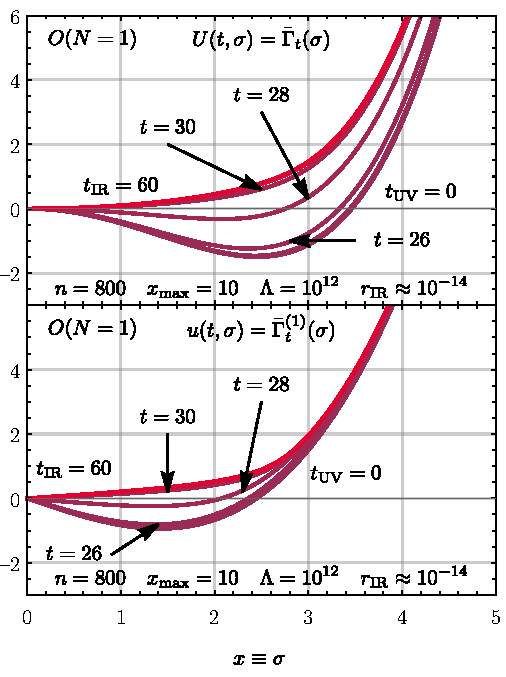
\includegraphics[width=\subcaptionFigureWidth-0.07cm]{0d/figures/sc_ii_n_on=1_n=800_xmax=10_lambda=1.0e12_tir=60_rg_flow.pdf}
		\caption{\frg{} flow of the effective potential $U ( t , \sigma )$ (upper panel) and its derivative $u ( t , \sigma ) = \partial_\sigma U ( t , \sigma )$ (lower panel)}
		\label{fig:sc_ii_n_on=1_n=800_xmax=10_lambda=1.0e12_tir=60_rg_flow}%
	}%
	{
		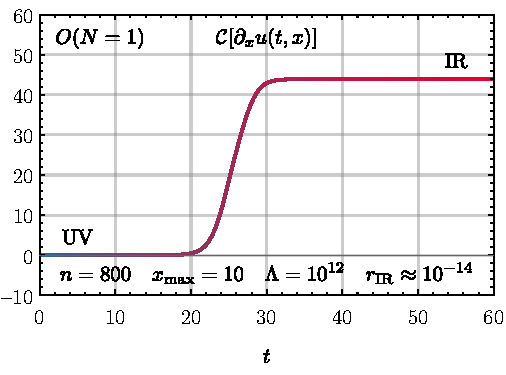
\includegraphics[width=\subcaptionFigureWidth]{0d/figures/sc_ii_n_on=1_n=800_xmax=10_lambda=1.0e12_tir=60_entropy_flow.pdf}
		\caption{\frg{} flow of the numerical entropy $\mathcal{C} [ \partial_x u ( t, x ) ]$}%
		\label{fig:sc_ii_n_on=1_n=800_xmax=10_lambda=1.0e12_tir=60_entropy_flow}%
	} % left figure
	{%
		\caption{
			\frg{} flow of the effective potential and its derivative on the top \subref{fig:sc_ii_n_on=1_n=800_xmax=10_lambda=1.0e12_tir=60_rg_flow} and corresponding flow of the numerical entropy below~\subref{fig:sc_ii_n_on=1_n=800_xmax=10_lambda=1.0e12_tir=60_entropy_flow} for the zero-dimensional $O(1)$ model with initial condition \eqref{eq:testing_scenario_phi4} with negative mass term.
			{Blue} color is associated to the \uv{} and {red} color to the \ir{}.
			We used the exponential regulator \cref{eq:exponential_regulator} with \uv{} scale $\Lambda = 10^{12}$.
			\fromFigs{3 and 5}{zerod2}
		}\label{fig:sc_ii_n_on=1_n=800_xmax=10_lambda=1.0e12_tir=60}
	}
	{\fullWidthTwoColumnFigureSpacing}
	{%
		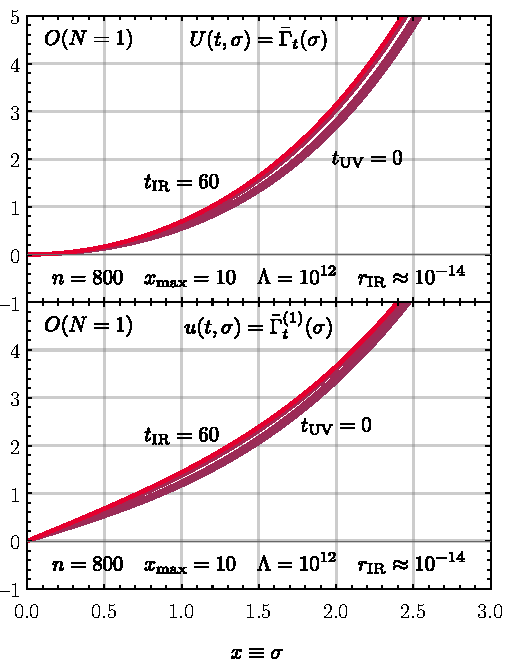
\includegraphics[width=\subcaptionFigureWidth]{0d/figures/sc_ii_p_on=1_n=800_xmax=10_lambda=1.0e12_tir=60_rg_flow.pdf}
		\caption{\frg{} flow of the effective potential $U ( t , \sigma )$ (upper panel) and its derivative $u ( t , \sigma ) = \partial_\sigma U ( t , \sigma )$ (lower panel).}
		\label{fig:sc_ii_p_on=1_n=800_xmax=10_lambda=1.0e12_tir=60_rg_flow}%
	}%
	{
		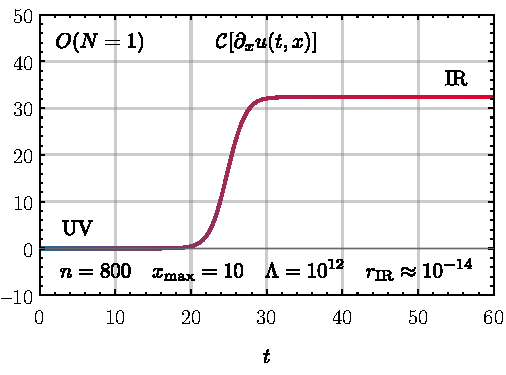
\includegraphics[width=\subcaptionFigureWidth-0.02cm]{0d/figures/sc_ii_p_on=1_n=800_xmax=10_lambda=1.0e12_tir=60_entropy_flow.pdf}
		\caption{\frg{} flow of the numerical entropy $\mathcal{C} [ \partial_x u ( t, x ) ]$}%
		\label{fig:sc_ii_p_on=1_n=800_xmax=10_lambda=1.0e12_tir=60_entropy_flow}%
	} % left figure
	{%
		\caption{
			\frg{} flow of the effective potential and its derivative on the top \subref{fig:sc_ii_p_on=1_n=800_xmax=10_lambda=1.0e12_tir=60_rg_flow} and corresponding flow of the numerical entropy below~\subref{fig:sc_ii_p_on=1_n=800_xmax=10_lambda=1.0e12_tir=60_entropy_flow} for the zero-dimensional $O(1)$ model with initial condition \eqref{eq:testing_scenario_phi4} with positive mass term.
			{Blue} color is associated to the \uv{} and {red} color to the \ir{}.
			We used the exponential regulator \cref{eq:exponential_regulator} with \uv{} scale $\Lambda = 10^{12}$.
			\fromFigs{4 and 6}{zerod2}
		}\label{fig:sc_ii_p_on=1_n=800_xmax=10_lambda=1.0e12_tir=60}
	}%
	[]\FloatBarrier
\paragraph{Test case II: \texorpdfstring{$\phi^4$}{phi**4} potential}\phantomsection\label{paragraph:sc2O1}\mbox{}\\%		
We continue our discussion of $O(1)$ models with test case II \eqref{eq:testing_scenario_phi4} with positive and negative mass term, recall \cref{fig:sc_ii_n_uv_initial_condition} for a visualization of this \ic{} with a negative mass term.
Depending on the sign of the mass term, we either start the \frg{} flow with a broken or restored \ZII{} symmetry.

When considering \cref{eq:testing_scenario_phi4} with negative mass term, we argued in \cref{paragraph:sc2taylorFlow} that during the \frg{} flow, while the physical point moves from $\sigma = \pm \sqrt{6}$ to $\sigma = 0$, presumably an excessively large or even infinitely many new couplings are generated in $U ( t, \sigma )$. 
This renders \frg{} Taylor expansion discussed in \cref{paragraph:sc2taylorFlow} at a finite order a potentially problematic approximation scheme for the evolution of non-convex potentials, see also \cref{subsubsec:sc3}.
In this paragraph, we reinforce our findings about the non-convergence of (Taylor) expansions of the potential during the \frg{} flow by studying the (numerical) entropy production during the \frg{} flows.

The \frg{} flows of $u ( t, x )$ for the \ic{} \eqref{eq:testing_scenario_phi4} with negative mass term is depicted in \cref{fig:sc_ii_n_on=1_n=800_xmax=10_lambda=1.0e12_tir=60_rg_flow} and \cref{fig:sc_ii_p_on=1_n=800_xmax=10_lambda=1.0e12_tir=60_rg_flow} shows the corresponding \frg{} flow\footnote{%
	Note that the plot range $x\in[0,3]$ for the ``positive mass''-case  differs from the one ($x\in[0,5]$) used in all other plots of \frg{} flows of $u ( t, x )$ in this subsubsection. 
	This is necessary to make the tiny changes during the \frg{} flow at least somewhat visible.
} for positive mass term.
Both \frg{} flows are by visual inspection not really spectacular: For the ``negative mass''-case, we find that, according to the \cmwhTheoremWithRefs{}, the diffusion via the \sigmaMode{} again restores the \ZII{} symmetry and drives the potential convex during the \rg{} flow before the system equilibrates in the \ir{}.
For the \frg{} flow of the ``positive mass''-case we only find minimal changes in the shape of $u ( t, x )$ also originating from the non-linear diffusion during the \frg{} flow.
Hence, the equilibrated solution in the \ir{} is relatively close to the \uv{} initial potential.\bigskip
	
The plots of the corresponding entropies in \cref{fig:sc_ii_n_on=1_n=800_xmax=10_lambda=1.0e12_tir=60_entropy_flow} (for negative mass term) and \cref{fig:sc_ii_p_on=1_n=800_xmax=10_lambda=1.0e12_tir=60_entropy_flow} (for positive mass term) are more instructive.
In both cases we find a clear monotonic rise of the (numerical) entropy exactly in the \frg{} time period, in which most of the dynamics takes place.
Furthermore, we clearly find plateaus in the \uv{} and the \ir{}, which correspond to the trivial \uv{} regime and the non-trivial interacting \ir{} regime.
This plateau-like behavior signals \rgcy{}.
In comparison with our first test case \eqref{eq:testing_scenario_non-analytic_quadaratic_asymptote}, where we used exactly the same discretization points (volume cells), the monotonic growth of entropy is less drastic and significantly smaller.
This is expected because the jumps in $u ( t = 0, x )$ at $x = 2$ and $x = 3$ in the first test case \eqref{eq:testing_scenario_non-analytic_quadaratic_asymptote} lead to greater changes in the discrete total variation \dash{} the arc length in $x$ of $u ( t, x )$ \dash{} than the rather small changes of the profiles of $u ( t, x )$ for the $\phi^4$-models, \cf{} \cref{paragraph:discrete_c_and_tvd}. 
Also from a fluid-dynamic perspective, this is intuitively understandable because the smoothening of huge gradients is a substantial source of entropy and obviously an irreversible process, whereas only a small transport of a fluid is not a source of excessive but rather small entropy production, even though it is diffusion driven.
Still, also for both $\phi^4$-cases the entropy increases during the \frg{} flow, which first signals an increasing number of coupling constants generated during the \frg{} flow, and second also renders the flows irreversible.
	
The second observation has severe consequences: Any \frg{} flow in a \frg{} Taylor expansion employs a finite set of coupled \odes{} for the couplings (vertices).
Since the system is finite, it seems to be theoretically possible integrate in either \rgtime{}-direction. 
In higher dimensions, one can formally integrate to larger scales when considering the perturbative beta functions of \qcd{}, \qed{}, \etc{}~\cite{Politzer:1973fx,Gross:1973id,Gross:1973ju,Gross:1974cs}, \cf{} \cref{paragraph:qcdAS}.
However, this is in principle not compatible with the irreversibility of \grg{} flows as shown in our present work (as, \eg{}, signaled by the rise of entropy)  and may only be reliable within small subspaces of the theory space associated with a given theory.
In fact, the computation of fundamental couplings at small scales (high energies) from effective couplings at large scales (low energies) is in general not possible, \cf{}\ \ccite{Wilson:1979qg}. We conclude that the increase of entropy, which we also observe during the \frg{} flow of our analytic initial conditions \eqref{eq:testing_scenario_phi4} reveals potential limitations of Taylor expansion of effective actions because most likely an extremely large (or even infinite) number of couplings is generated in the \frg{} flow and would be required to correctly describe the \frg{} flow 
\footnote{%
	At this point, one might be tempted to apply our definition of the normalized (numerical) entropy directly to some $\partial_x u ( t, x )$ that is reconstructed from the flow of the coefficients of a Taylor expansion of the potential to study the validity of the expansion.
	However, this is not possible, because the \frg{} Taylor expansion in general provides only an adequate local description of the potential, while our (numerical) entropy or the \tv{} requires knowledge about the global shape of the potential or its derivatives.
}.%

When considering an expansion in vertices (especially in higher/non-zero dimensions), it might be possible that higher-order couplings/vertices are strongly suppressed (especially when considering higher-dimensional \qfts{}), 
such that an expansion of the \frgEquation{} in vertices is applicable and meaningful in practice, see, \eg{}, \ccite{Eser:2018jqo,Eser:2019pvd,Divotgey:2019xea,Cichutek:2020bli}.
This should go hand in hand with only a small growth of an entropy for the exact \frg{} flow.
Exactly this seems to be the case for our ``positive mass'' case \eqref{eq:testing_scenario_phi4}, which shows almost no dynamics at all and yields the smallest increase in entropy of all our test cases. 
A reason, why here a rather small number of couplings might be sufficient to describe the entire \frg{} flow is that the potential is convex during the entire flow and has a single unique non-moving minimum.
Hence, the \uv{} regime of this model and the \ir{} regime do not differ much and, as long as the quartic coupling is extremely small, also perturbation theory~\cite{Strocchi:2013awa} leads to results which are consistent with the exact values for the lowest \ipi{} \nptFunctions{}~\cite{Keitel:2011pn}.

\fullWidthTwoColumnTwoSubFigures{%
		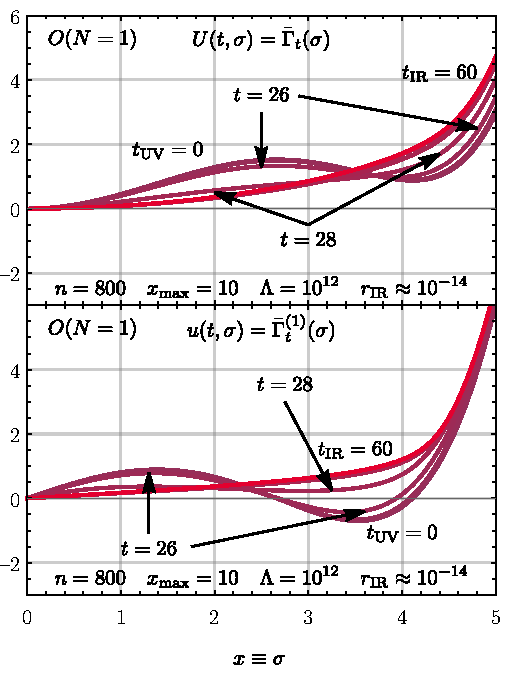
\includegraphics[width=\subcaptionFigureWidth-0.015cm]{0d/figures/sc_iii_on=1_n=800_xmax=10_lambda=1.0e12_tir=60_rg_flow.pdf}
		\caption{\frg{} flow of the effective potential $U ( t , \sigma )$ (upper panel) and its derivative $u ( t , \sigma ) = \partial_\sigma U ( t , \sigma )$ (lower panel).}
		\label{fig:sc_iii_on=1_n=800_xmax=10_lambda=1.0e12_tir=60_rg_flow}%
	}%
	{
		\vspace{-0.01cm}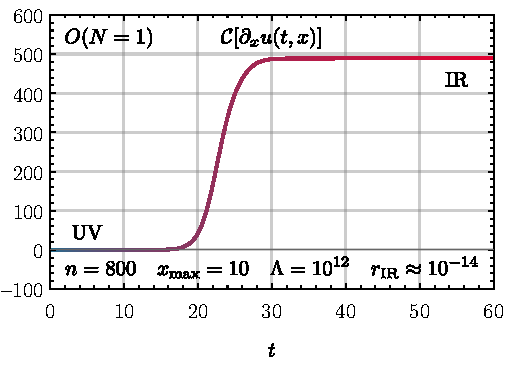
\includegraphics[width=\subcaptionFigureWidth]{0d/figures/sc_iii_on=1_n=800_xmax=10_lambda=1.0e12_tir=60_entropy_flow.pdf}
		\caption{\frg{} flow of the numerical entropy $\mathcal{C} [ \partial_x u ( t, x ) ]$}%
		\label{fig:sc_iii_on=1_n=800_xmax=10_lambda=1.0e12_tir=60_entropy_flow}%
	} % left figure
	{%
		\caption{
			\frg{} flow of the effective potential and its derivative on the top \subref{fig:sc_iii_on=1_n=800_xmax=10_lambda=1.0e12_tir=60_rg_flow} and corresponding flow of the numerical entropy below~\subref{fig:sc_iii_on=1_n=800_xmax=10_lambda=1.0e12_tir=60_entropy_flow} for the zero-dimensional $O(1)$ model with initial condition \eqref{eq:testing_scenario_phi6}.
			{Blue} color is associated to the \uv{} and {red} color to the \ir{}.
			We used the exponential regulator \cref{eq:exponential_regulator} with \uv{} scale $\Lambda = 10^{12}$.
			\fromFigs{7 and 8}{zerod2}
		}\label{fig:sc_iii_on=1_n=800_xmax=10_lambda=1.0e12_tir=60}
	}%
	{\fullWidthTwoColumnFigureSpacing}%
	{%
		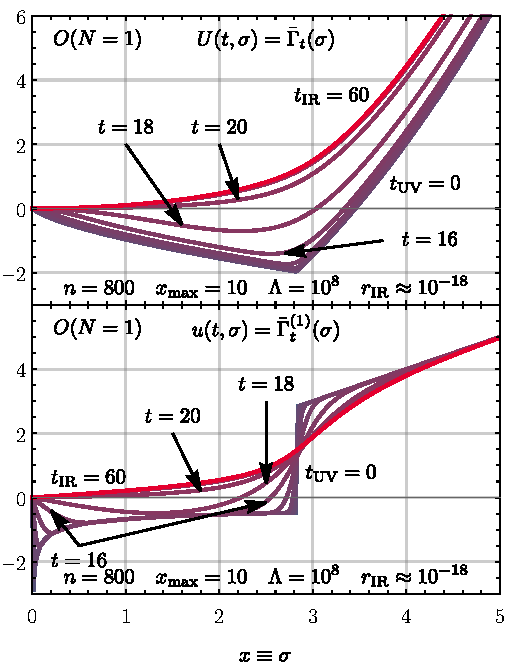
\includegraphics[width=\subcaptionFigureWidth]{0d/figures/sc_iv_on=1_n=800_xmax=10_lambda=1.0e8_tir=60_rg_flow.pdf}
		\caption{\frg{} flow of the effective potential $U ( t , \sigma )$ (upper panel) and its derivative $u ( t , \sigma ) = \partial_\sigma U ( t , \sigma )$ (lower panel).}
		\label{fig:sc_iv_on=1_n=800_xmax=10_lambda=1.0e8_tir=60_rg_flow}%
	}%
	{
		\vspace{0.05cm}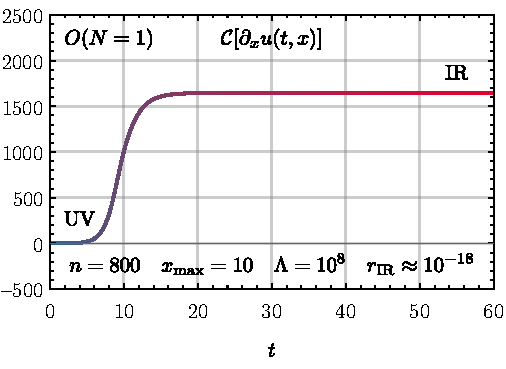
\includegraphics[width=\subcaptionFigureWidth-0.01cm]{0d/figures/sc_iv_on=1_n=800_xmax=10_lambda=1.0e8_tir=60_entropy_flow.pdf}
		\caption{\frg{} flow of the numerical entropy $\mathcal{C} [ \partial_x u ( t, x ) ]$}%
		\label{fig:sc_iv_on=1_n=800_xmax=10_lambda=1.0e8_tir=60_entropy_flow}%
	} % left figure
	{%
		\caption{
			\frg{} flow of the effective potential and its derivative on the top \subref{fig:sc_iv_on=1_n=800_xmax=10_lambda=1.0e8_tir=60_rg_flow} and corresponding flow of the numerical entropy below~\subref{fig:sc_iv_on=1_n=800_xmax=10_lambda=1.0e8_tir=60_entropy_flow} for the zero-dimensional $O(1)$ model with initial condition \eqref{eq:testing_scenario_4}.
			{Blue} color is associated to the \uv{} and {red} color to the \ir{}.
			We used the exponential regulator \cref{eq:exponential_regulator} with \uv{} scale $\Lambda = 10^8$.
			\fromFigs{9 and 10}{zerod2}
		}\label{fig:sc_iv_on=1_n=800_xmax=10_lambda=1.0e8_tir=60}
	}%
	[]
\FloatBarrier
\paragraph{Test case III: \texorpdfstring{$\phi^6$}{phi**6} potential}\phantomsection\label{paragraph:sc3O1}\mbox{}\\%		 
We continue our discussion of $O(1)$ models with test case III \eqref{eq:testing_scenario_phi6}, recall \cref{fig:sc_iii_uv_initial_condition} for a visualization of this \ic{}.
In \cref{paragraph:sc3taylorConclusion}, we came to the conclusion that there has to be a time interval during the \frg{} flow, where $u ( t, x )$ exhibits highly non-local dynamics \dash{} preventing the applicability of a Taylor expansion, even though the expansion point is unique and does not move.
The \frg{} flows of $u ( t, x )$ for \eqref{eq:testing_scenario_phi6} with negative mass term is depicted in \cref{fig:sc_iii_on=1_n=800_xmax=10_lambda=1.0e12_tir=60_rg_flow}.

At $t \approx 27$ the local minimum (the second non-trivial zero-crossing) vaporizes via the diffusion and merges with the local maximum.
It is this dynamics which triggers the breakdown of the Taylor expansion manifesting as strongly oscillating and ultimately diverging couplings at $t \approx 27$. \bigskip

Interestingly, also the (numerical) entropy function signals exactly the discussed non-local behavior at $t \approx 27$.
At that point in time, when the local minimum vaporizes, we observe the strongest increase of entropy, see \cref{fig:sc_iii_on=1_n=800_xmax=10_lambda=1.0e12_tir=60_entropy_flow}.
We also find that by absolute measures, the entropy production for the $\phi^6$-initial potential \eqref{eq:testing_scenario_phi6} is greater than the entropy production observed for both quartic initial conditions~\eqref{eq:testing_scenario_phi4}.
Nevertheless, the entropy production for the non-analytic initial condition~\eqref{eq:testing_scenario_non-analytic_quadaratic_asymptote} is still greater than the one in the $\phi^6$-case.
This can be understood from the relation of the numerical entropy to the \tv{}, \ie{}, the arc length of $u ( t, x )$ which even formally diverges for \cref{eq:testing_scenario_non-analytic_quadaratic_asymptote} in the \uv{}, keeping in mind that a comparison of absolute values of the numerical entropy should be considered with some care, \cf{} \cref{paragraph:discrete_c_and_tvd}.
	
We conclude this paragraph noting that that the (numerical) entropy might be a useful measure for deciding whether a system at a given \rgscale{}/time is in a perturbative or non-perturbative regime.
In other words, it is a tool to discuss whether the \frg{} flow is governed by strong (non-perturbative) dynamics or by weak (perturbative) dynamics.
The \cfd{} analogy to this situation would be the difference between a fluid evolving through an out-of-equilibrium state, before finally equilibrating or showing steady-flow behavior, in contrast to a fluid that is already close to its equilibrium state.

\paragraph{Test case IV: The \texorpdfstring{$\sigma = 0$}{sigma=0} boundary}\phantomsection\label{paragraph:sc4O1}\mbox{}\\%
We conclude our discussion of explicit numerical results for the $O(1)$ model with test case IV~\eqref{eq:testing_scenario_4}, recall \cref{fig:sc_iv_uv_initial_condition} for a visualization of this \ic{}.
The test case~\eqref{eq:testing_scenario_4} turns out to be a highly interesting almost pathological example in this context.
The \frg{} flow of $u ( t, x )$ is shown in \cref{fig:sc_iv_on=1_n=800_xmax=10_lambda=1.0e8_tir=60_rg_flow}.

Of specific interest regarding the (numeric) entropy is of course the pole of $u ( t = 0, x )$ at $x = 0$.
Formally, the arc length of $u ( t, x )$, which is directly related to our entropy function, diverges due to the pole at $x = 0$ for all $t > 0$.
This divergence is of different nature than the divergence caused by integrating from $x = - \infty$ to $x = + \infty$ in \cref{eq:entropy_func}.
Whereas the latter can be cured by normalizing the entropy \wrt{} the entropy of $u ( t = 0, x)$, the present divergence also occurs on the level of the ``normalized''  entropy function \eqref{eq:Cdef} similar to the other non-analytic jumps in the \uv{}.
The reason for the infinite entropy production while going from $t = 0$ to $t > 0$ is exactly that the total variation between $- x_{\mathrm{max}}$ and $+ x_{\mathrm{max}}$ turns finite for $u ( t, x )$ during the flow because the potential turns convex and smooth.
Moreover, symmetry restoration in the ground state sets in for $t \rightarrow \infty$.
However, it is still normalized against the infinite total variation of $u ( t = 0, x )$.
Interestingly, this problem can be traced back to the initialization of the \frg{} flow equations at $t = 0$ with the classical \uv{} action $\bar{\Gamma}_{t = 0} ( \varphi ) = \mathcal{S} ( \varphi )$, which is actually not totally exact but rather an almost perfect approximation for sufficiently large $\Lambda$, see also our discussion in \cref{subsubsec:zerodICS}.
However both the inherent diffusive nature of the \frg{} flow equation and the employed finite-volume discretization render the pole at $\sigma = 0$ a huge but already finite jump captured in three volume cells on the level of the cell averages $\bar{u}_i ( t )$ at $t = 0$.
Therefore, we can use $u ( t = 0, x )$ as our reference entropy for the normalization of \cref{eq:Cdef} as it is numerically finite right from the beginning of the flow.\bigskip

The explicit result for the \frg{} flow of our (numerical) entropy is shown in \cref{fig:sc_iv_on=1_n=800_xmax=10_lambda=1.0e8_tir=60_entropy_flow}.
Irrespective of the subtleties of the preceding discussion, we find a rather large entropy production at exactly those times when the pole vanishes and the jumps at $x = \pm \sqrt{8}$ are smeared out via the diffusion.

Additionally, we find that the total entropy production is much larger for this test case than for the previous ones. Again, this is of course directly related to the huge gradients in the initial condition, which are tremendous sources of entropy via dissipation, directly analogous to the \he{} discussed in \cref{paragraph:HE}.\bigskip

In this subsubsection, we confronted our theoretical findings of \cref{subsubsec:0dO1entropy_c-function_tvd} with direct numerical computations using the \ktScheme{}.
We verified the behavior of the function $\mathcal{C} [ \partial_x u ( t, x ) ]$ from \cref{eq:Cdef} by means of its discretized version in \cref{eq:Cdiscrete} as a valid numerical entropy measure in four test cases.
Using the numerical entropy and the Wetterich equation in the form~\eqref{eq:o(1)_wetterich_equation}, we made several, at this point almost intuitive, connections between phenomena known in fluid- and thermodynamic processes and directly related processes and aspects of \grg{} flows.
Most notable, the diffusive character of the flow equation~\eqref{eq:o(1)_wetterich_equation} results directly in irreversible \frg{} flows.
This also establishes a connection between steady-state/(thermal) equilibrium solutions and the \uv{}  and \ir{} regime.
Moreover, the application of the numerical entropy and total variation appears to be an attractive monitor for \rgcy{} and the origin of an ``thermodynamic'' time asymmetry.

\subsubsection{Irreversibility of the RG flow, entropy, and the \texorpdfstring{$\mathcal{C}$}{C}-theorem}
\label{subsubsec:c-theorem_irreversibility_entropy}
\begin{disclaimer}
	This subsubsection summarizes and references the findings of Sec. V of \ccite{Koenigstein:2021rxj}.
	The \customref{paragraph:cTheoremzerodO1}{first paragraph} of this subsubsection includes material for the Virasoro algebra and fixed-point solutions for the zero-dimensional \ONn{1} from the unpublished notes~\cite{Koenigstein:fixedPoint}.
\end{disclaimer}
The (re)discoveries within this work unravel the connection between the (numerical) entropy and total variation, employed in applied mathematics, and the irreversibility inherent to \grg{} flows. Furthermore, they might even provide some connections to $\mathcal{C}$-/$\mathcal{A}$-theorems within the framework of truncated \frg{} flow equations. 

The original formulation of Zamolodchikov's $\mathcal{C}$-theorem~\cite{Zamolodchikov:1986gt} states that for a two-dimensional field theory the following properties hold:
\begin{enumerate}
	\item There exists a positive function 
		\begin{align}
			\mathcal{C} ( \{ g_i \}, t ) \geq 0 \, ,	\label{eq:c-function_1}
		\end{align}
	of all (possibly infinitely many) dimensionless couplings $\{ g_i \}$ of the theory and \rgtime{} $t$, with the additional property
		\begin{align}
			+\dod{}{t} \mathcal{C} ( \{ g_i \}, t ) \geq 0 \, ,	\label{eq:c-function_2}
		\end{align}
	where the choice of sign in front of the derivative is convention.
	
	\item The $\mathcal{C}$-function takes a fixed value at (critical) fixed points $g_i^\ast$ of the theory:
		\begin{align}
			\mathcal{C} ( \{ g_i^\ast \}, t ) = c_i \, ,	\label{eq:c-function_3}
		\end{align}
	where the fixed value $c_i$ can be identified with the central charge $c$ (giving  the $\mathcal{C}$-theorem its name) of a \textit{Virasoro algebra}~\cite{Virasoro:1969zu}
		\begin{align}
			\big[ L_m, \, L_n \big] = L_m L_n - L_n L_m = \,& ( m - n ) \, L_{m + n} + \frac{c}{12} \, ( m^3 - m ) \, \delta_{m + n, 0} \, ,	\label{eq:c-function_virasoro}
		\end{align}
	with the generators $L_n$ of the infinite conformal group.
	The central charge is different for different fixed points.
\end{enumerate}
$\mathcal{C}$-theorems and their generalizations especially from two to four dimensions $\mathcal{A}$-theorems~\cite{Cardy:1988cwa} are still under active research, see, \eg{}, \ccite{Zamolodchikov:1986gt,Rosten:2010vm,Banks:1987qs,Cardy:1988cwa,Osborn:1989td,Jack:1990eb,Komargodski:2011vj,Curtright:2011qg,Haagensen:1993by,Generowicz:1997he,Forte:1998dx,Codello:2013iqa,Codello:2015ana,Becker:2014pea,Becker:2016zcn}.
$\mathcal{A}$-theorems get their name from anomaly coefficients which are proposed to take the role of the central charge in four dimensions.
A general overview of this field is beyond the scope of the current work and we will focus in the following paragraphs on specific aspects relevant to this work and the \frg{}.

One other interesting aspect, related to the introduction of a numeric entropy for \frg{} flows, was pointed out by the referee of \ccite{zerod2}: the present formulation based on the effective potential shares some similarities with the macroscopic description of systems in statistical mechanics.
Instead of working with an infinite set of couplings (microstates in statistical mechanics) we switch to a description in terms of an effective potential (a macroscopic formulation in statistical mechanics).
The inability (of a macroscopic observer) to track the dynamics of an infinite set of couplings (microstates in statistical mechanics) leads to a macroscopic entropy production/information loss and irreversible processes.
An approach to formalize this notion in statistical mechanics was made by Ludwig Boltzmann~\cite{Boltzmann2003} and later Josiah W. Gibbs~\cite{Gibbs2010Sep} with the introduction of $H$-theorems, see, \eg{}, Chap. VI and XII of the textbook~\cite{Tolman1979Nov} for further details. Exploring this connection and possible relations between  $\mathcal{C}$-/$\mathcal{A}$- and $H$-theorems further could be a very interesting prospect for further research.

\paragraph{The \texorpdfstring{$\mathcal{C}$}{C}-theorem of the zero-dimensional \texorpdfstring{\ONn{1}}{O(1)} model}\phantomsection\label{paragraph:cTheoremzerodO1}\mbox{}\\%
In this paragraph we will argue that our numerical entropy \eqref{eq:Cdef} for the zero-dimensional \ONn{1} model is in fact a direct analogon to Zamolodchikov's $\mathcal{C}$-function in zero dimensions.
Our numerical entropy \eqref{eq:Cdef} fulfills the first two defining properties \eqref{eq:c-function_1} and \eqref{eq:c-function_2} by construction.
$\mathcal{C} [ \partial_x u ( t, x ) ]$ and its \fv{} equivalent $\mathcal{C} [ \{\bar{u}_j(t)\}]$ are also functions of all (infinitely many) coupling constants which are dimensionless in ${d=0}$ and encoded via $u ( t, x )$ or equivalently in \fv{} discretization in the set of volume averages $\{\bar{u}_j(t)\}$.

The only open question regarding the interpretation of our numerical entropy \eqref{eq:Cdef} as a $\mathcal{C}$-theorem is related to the question of fixed points and the central charge.
\Apriori{} it is difficult to just imagine a meaningful zero-dimensional analog of central charge and conformal symmetry.
\Aposteriori{} \dash{} after an extensive review of the literature of zero-dimensional \qfts{} and specifically zero-dimensional \ON{} models \dash{} there might be a meaningful analogon for the central charge, \ie{}, the absence of such charges, in zero dimension.
S. Nishigaki and T. Yoneya in \ccite{Nishigaki:1990sk}  and P. Di Vecchia, M. Kato, and N. Ohta in \ccite{DiVecchia:1990ce} observe, that it is possible to derive \dses{} for the zero-dimensional $O(N)$ model which can be recast into a Virasoro algebra.
Following \ccite{Nishigaki:1990sk} we consider the partition function $\mathcal{Z}$ as a function of all, infinitely many couplings $\{\lambda_j\}$ of a zero-dimensional \ON{} model
\begin{align}
	\mathcal{Z} ( \{\lambda_j\} ) \equiv \int \dif^{\,N}\! \phi \, \exp \bigg[ - \sum_{j = 1}^{\infty} \lambda_j \, ( \vec{\phi}^{\, 2} \, )^j \bigg]\,.\label{eq:zerodO1Zdse}
\end{align}
From the divergence theorem, we find for $n \in \Integers{}_0$
\begin{align}
	0 = \, & \int \dif^{\,N}\! \phi \, \frac{\partial}{\partial \phi^i} \bigg( \phi^i \, ( \vec{\phi}^{\, 2} )^n \, \exp \bigg[ - \sum_{j = 1}^{\infty} \lambda_j \, ( \vec{\phi}^{\, 2} \, )^j \bigg] \bigg)\, ,
\end{align}
%For $n = 0$, we find
	%\begin{align}
		%0 = \, & \bigg( \tfrac{N}{2} + \sum_{j = 1}^{\infty} j \, \lambda_j \, \frac{\partial}{\partial \lambda_j} \bigg) \, \mathcal{Z} ( \vec{\lambda} \, ) \, ,
	%\end{align}
%while for $n \geq 1$
	%\begin{align}
		%0 = \, & \bigg[ - \big( \tfrac{N}{2} + n \big) \, \frac{\partial}{\partial \lambda_n} + \sum_{j = 1}^{\infty} j \, \lambda_j \, \frac{\partial}{\partial \lambda_{j + n}} \bigg] \, \mathcal{Z} ( \vec{\lambda} \, ) \, ,
	%\end{align}
%where we additionally divided by a factor of two.
which when evaluated for $n=0$ and $n \geq 1$ allow for the definition of 
\begin{align}
	L_n \equiv \, & - \big( \tfrac{N}{2} + n \big) \, \frac{\partial}{\partial \lambda_n} + \sum_{j = 1}^{\infty} j \, \lambda_j \, \frac{\partial}{\partial \lambda_{j + n}} \label{eq:zerodO1L}
\end{align}
such that
\begin{align}
	0 = L_n \, \mathcal{Z} ( \{\lambda_j\} ) \, .\label{eq:zerodO1dse}
\end{align}
These operators $L_n$ form an algebra
\begin{align}
	\big[ L_m, \, L_n \big] = \, & ( m - n ) \bigg[ - \big( \tfrac{N}{2} + m \big) \, \frac{\partial}{\partial \lambda_{m + n}} +  \sum_{i = 1}^{\infty} i \, \lambda_i \, \frac{\partial}{\partial \lambda_{i + m + n}} \bigg] = \, ( m - n ) \, L_{m + n} \, ,\label{eq:c-function_witt}
\end{align}
which is a Virasoro algebra \eqref{eq:c-function_virasoro} with vanishing central charge $c$, \ie{}, a so-called \textit{Witt algebra}~\cite{Witt1937Jan}.
The \dses{} \eqref{eq:zerodO1dse} for $\mathcal{Z} ( \{\lambda_j\} )$ inform and establish the Witt algebra \eqref{eq:c-function_witt}, \ie{}, a Virasoro algebra with vanishing central charge, for the zero-dimensional \ON{} model.
Following Zamolodchikov and assuming that the operators for the \dses{} $L_n$ from \cref{eq:zerodO1L} are a meaningful zero-dimensional analogon to the generators $L_n$ of the infinite conformal group in two dimensions, one would assume that \cref{eq:c-function_witt} implies an absence of fixed-point solutions in zero-dimensional \ON{} models.

We will prove the latter for the zero-dimensional \ONn{1} model explicitly.
We start from the \frg{} flow equation \eqref{eq:o(1)_wetterich_equation} by reformulating the equation at finite \rgtime{} in terms of the regulator itself
\begin{align}
	\partial_r u ( r, x ) = \frac{1}{2} \, \dod{}{x} \frac{1}{r + \partial_x u ( r , x )} \, ,
\end{align}
which in turn may be rewritten using the substitution $u ( r, x ) \equiv w ( r, x ) - r \, x$:
\begin{align}
	\partial_r w ( r, x ) - x = \, & \frac{1}{2} \, \dod{}{x} \frac{1}{\partial_x w( r , x )}\, .
\end{align}
Hence, the global fixed-point equation (with $\partial_r w ( r, x )=0$) reads
\begin{align}
	- x = \frac{1}{2} \, \dod{}{x} \frac{1}{\partial_x w ( r , x )}\,,
\end{align}
which can be integrated to
\begin{align}
	x_0^2 - x^2 = \frac{1}{\partial_x w ( r, x )} - \frac{1}{\partial_{x_0} w ( r, x_0 )}
\end{align}
The potential $U ( r, x )$ has to be \ZII{}-symmetric and convex for all $r$, if it is supposed to be an admissible global fixed-point solution.
Thus, $\partial_x w ( r, x )$ has to be positive for all $x_0 \neq 0$. 
As long as we choose $x_0 \in ( 0, \pm \infty )$, explicitly excluding $x_0 = 0$ and $x_0 = \pm \infty$, we can absorb both integration constants in a non-zero, positive integration constant, which we set \wlogA{} to unity in the following, and derive
\begin{align}
	\partial_x w ( r, x ) = \frac{1}{1 - x^2} \, .
\end{align}
This equation can be integrated to obtain
\begin{align}
	w ( r, x ) =
	\begin{cases}
		\mathrm{artanh} ( x ) \, ,	&	|x| < 1 \, ,
		\\
		\mathrm{arcoth} ( x ) \, ,	&	|x| > 1 \, ,
	\end{cases}\label{eq:zerodO1w}
\end{align}
which however implies, that there is only a convex solution to the fixed-point equation for $x \in ( - 1, + 1)$. 
In conclusion, a global convex fixed-point solution does not exist.
We may also note that the partition function \eqref{eq:partition_function} for the potential $U ( r, x ) = W ( r, x ) - \frac{1}{2} \, r \, x^2$ with the integral of \cref{eq:zerodO1w} does not converge since $\lim_{x\rightarrow \pm\infty}W(r,x)=1+\frac{1}{2}\ln(x^2)+\order(x^{-2})$.\bigskip

In summary we note that our numerical entropy \eqref{eq:Cdef} for the zero-dimensional \ONn{1} model is a proper analogon to  Zamolodchikov's $\mathcal{C}$-function. The following $\mathcal{C}$-theorem holds for the zero-dimensional \ONn{1} model: $\mathcal{C} [ \partial_x u ( t, x ) ]$ from \cref{eq:Cdef} and its discrete \fv{} equivalent $\mathcal{C} [ \{\bar{u}_j(t)\}]$ from \cref{eq:Cdiscrete} are positive and monotonically increasing during \frg{} flow and there are no global, convex fixed-point solutions with the Witt algebra~\eqref{eq:c-function_witt} for the \dses{}~\eqref{eq:zerodO1dse} as analogon to the Virasoro algebra~\eqref{eq:c-function_virasoro}.

\paragraph{The challenges of a generalization to finite $N>1$ in zero dimensions}\phantomsection\label{paragraph:cTheoremzerodON}\mbox{}\\%
To discuss the construction of a $\mathcal{C}$-function for $N>1$ we recall the \frg{} flow \cref{eq:advection_diffusion_equation_zero-dimensional} 
\begin{align}
	&\partial_t u + \dod{}{x} F [ t, x, u ] = \dod{}{x} Q [ t, \partial_x u ]\, ,
\end{align}
and its primitive form
\vspace{-.05em}
\begin{align}
&\partial_t u + \frac{\partial F [ t, x, u ]}{\partial u}  \, \partial_x u - \frac{\partial Q [ t, \partial_x u ]}{\partial(\partial_x u)} \partial_x^2 u ( t, x ) = -\partial_x F [ t, x, u ]\,.\label{eq:zerodO1primitive}
\end{align}
\vspace{-.05em}
\Cref{eq:zerodO1primitive} includes convective contributions on the \lhs{} but also an internal source term, stemming from the position-dependence of the advection flux, on the \rhs{}
We discussed such a situation in the general \cfd{} context in \cref{subsec:hydroAdvection} and implications for the \tv{} in \cref{subsec:hydroKT}: (internal) source terms lead to a loss of the \tvni{} property \dash{} they change and crucially increase \tv{}/arc length during time evolution.
Hence \tv{} is no longer a valid candidate for a numerical entropy functional, which in presence of sources is notoriously difficult to construct in a \cfd{} context, see, \eg{}, \ccite{Monthe:2001,Beneito2008,Chen2011May,Bessemoulin:2012} and references therein. 

The explicit position-dependence of the advection flux prevented us from formulating a numerical entropy for the zero-dimensional $O(N)$ model for finite $N > 1$.
The corresponding contribution to the entropy function \eqref{eq:Cdef} allows for $\tfrac{\dif}{\dif t} \, \mathcal{C} [ \partial_x u ( t, x ) ] < 0$ during \frg{} flow for certain initial conditions and $N$ in the case of $N > 1$.
For the zero-dimensional cases \eqref{eq:testing_scenario_phi4} and \eqref{eq:testing_scenario_phi6} discussed, we find $\tfrac{\dif}{\dif t} \, \mathcal{C} [ \partial_x u ( t, x ) ] < 0$ during the \rg{} evolutions for $N \geq 8$.
For the cases \eqref{eq:testing_scenario_non-analytic_quadaratic_asymptote} and \eqref{eq:testing_scenario_4} with their $\sigma^2$ asymptotics for large $\sigma$ the inequality $\tfrac{\dif}{\dif t} \, \mathcal{C} [ \partial_x u ( t, x ) ] \geq 0$ seems to hold for all $N$ and $t$.

Reformulating the \frg{} flow \cref{eq:conservation_law_u_phi} in the invariant $y\equiv \tfrac{1}{2} \, x^2$, \cf{} \cref{eq:conservation_law_u_rho}, does not solve the issue of internal source terms at finite $N$. 
While the advection flux in \cref{eq:conservation_law_u_rho} loses its explicit position-dependence the diffusion flux gains both a dependence on $u(t,y)$ and $y$ which does not improve our situation at finite $N$.
In the infinite-$N$ limit however diffusive contributions vanish after rescaling with $N-1$ and a formulation in $y$ with a $y$-independent advection flux allows for an identification of the \tv{} as an entropy functional.
We will discuss this in \cref{paragraph:infiniteNflowsEntropy}.

\vspace{-.65em}
\paragraph{Comments on a generalization to (higher-dimensional) \texorpdfstring{$O(N)$}{O(N)} models}\phantomsection\label{paragraph:cTheoremON}\mbox{}\\
A direct generalization of our findings regarding numerical entropy measures for the \frg{} flow from zero to non-zero dimensions is hindered by two new conceptual issues:
\begin{enumerate}
	\item The \lpa{} as part of the leading-order of a \de{} is in general only a truncation in $d>0$, \cf{} \deRef{}.
	This makes very general statements for the \qft{} under consideration \apriori{} impossible when just discussing the \frg{} flow of the potential.
	That being said the established concept of numerical entropy might still be of some use in higher-dimensional $O(1)$ models.
	\item	In contrast to the zero-dimensional model, the couplings in $d>0$ can have non-zero energy dimensions.
	Thus, our numerical entropy \eqref{eq:Cdef} cannot adequately describe the second property of the $\mathcal{C}$-theorem \eqref{eq:c-function_3} \dash{} namely capturing the properties of fixed points, which are defined via the zeroes of the beta functions of all dimensionless couplings and additionally a constant $\mathcal{C}$-/$\mathcal{A}$-function.
	To resolve the fixed-point structure, one has to consider the flow equation for rescaled quantities which gains additional internal source terms due to the rescaling, \cf{} Eq. (37) of \ccite{zerod2}.
	Such source terms make \tv-like entropy measures unviable.
\end{enumerate}
Further details can be found in Sec. V of \ccite{zerod2}.\clearpage